\chapter{Cheap Rate Mail}

Although the application of an adhesive postage stamp provides a covenient
means of prepaying for postage on a small number of letters, 
special handstamps were supplied to facilitate the handling of large batches of letters.

\ph[width = .80\textwidth]{../cape-of-good-hope/newspaperbranch/wrapper-1_2d-paid.jpg}{ 
}
<p style="font-family:arial;font-size:12px;float:left">Provenance: Y Lazarides</p><div style="clear:both"></div>


This is termed the 'Cheap Rate Mail'. These handstamps indicated the prepayment 
of postage in respect of the item on which they were impressed and dispensed 
with the need to affix a postage stamp.

\begin{marginfigure}
\centering
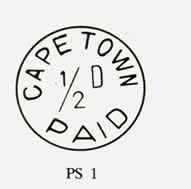
\includegraphics[width=.45\textwidth]{../cape-of-good-hope/cheap-rate-mail/cape-paid-1_2d.jpg}
\caption{Cheap Rate Handstamp Cape Town half penny.}
\end{marginfigure}


The first of the Paid Stamps (PS 1) to denote prepayment of postage during
 the adhesive period, was brought into use about 1870. 
 It was cirular, with a diameter of 24 mm. It contains the words "Cape Town" 
 and "Paid" within the circle with$\frac{1}{2}$ d denomination at the centre. 
 Golblatt records tha this was the only value used, the strike 
 always being impressed in red, however, a 1d 'Paid' stamp of a 
 similar design exists.This is illustrated below and referred to as (PS 1 a). 
 The$\frac{1}{2}$ d being used for postcards and the 1 d for newspapers.

\begin{marginfigure}
\centering
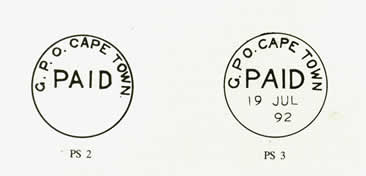
\includegraphics[width=.95\textwidth]{../cape-of-good-hope/cheap-rate-mail/paid-stamps.jpg}
\caption{Cheap Rate Handstamps with no value markings.} 
\end{marginfigure}

In 1888 a new design (PS 2) came into use in the Cape of Good Hope. 
It was also of a circular design and had a diameter of 30 mm. 
It had the wording G.P.O. Cape Town ontop and in the middle, 
in large type the word 'Paid'.


\ph[width = .80\textwidth]{../cape-of-good-hope/cheap-rate-mail/1d-paid-wrapper.jpg}{
Wrapper with two unrecorded marks. Deficiency Noted and a 1d PAID cds.\label{deficiency}}

In my collection I have a wrapper shown in \ref{deficiency}, of a  Cape Times (weekly edition) with two unusual and unreported marks. The circular paid mark is similar to \postmark{PS1}, as classified by Goldblatt, however Goldblatt reports that only the$\frac{1}{2}$d denomination was used. The wrapper bears a rectangular shape mark with the wording \textsc{defficiency noted}, which is also not reported by Goldblatt. The mark is unlikely to be a tax mark, but rather indicates that the contents were probably partially missing or were damaged.

In 1907 a similar design to Paid 
Stamps PS 2 and PS 3 this was issued (PS 3) with slightly smaller 
lettering and this had the date, month and year at the bottom. 
These types are found struck both in black as well as red ink. Most of these continued  to be used after the Union Of South Africa.

\subsubsection{References}


1  \goldblatt{128}


                                                        